%----------------
\begin{figure*}
  \centering
  \subfloat[\covtype]{
  		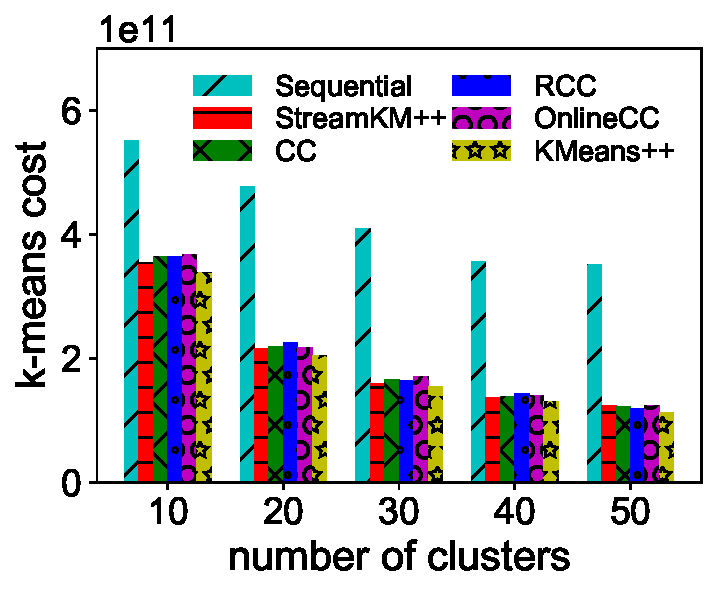
\includegraphics[width=0.24\textwidth]{expfigs/accuracy_k/covtype_cost_vs_k.pdf}
  }
  \subfloat[\power]{
  		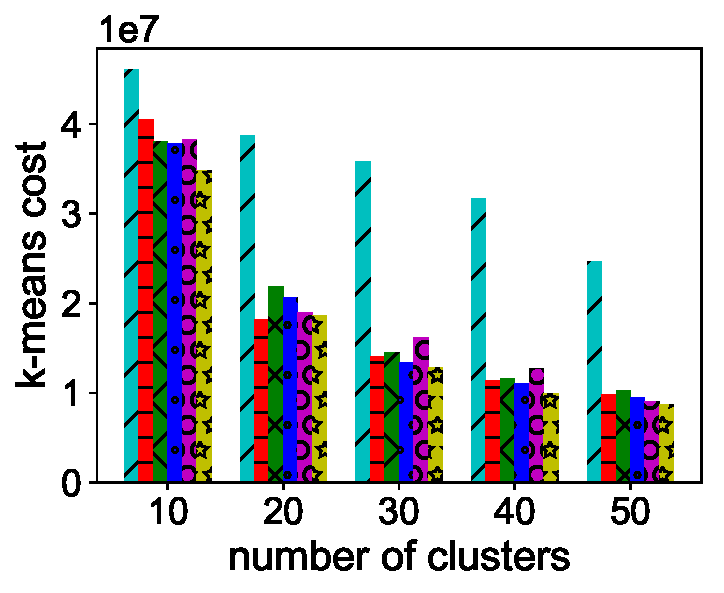
\includegraphics[width=0.24\textwidth]{expfigs/accuracy_k/power_cost_vs_k.pdf}
  }
  \subfloat[\intrusion (\km cost of \seqkm is not shown)]{
		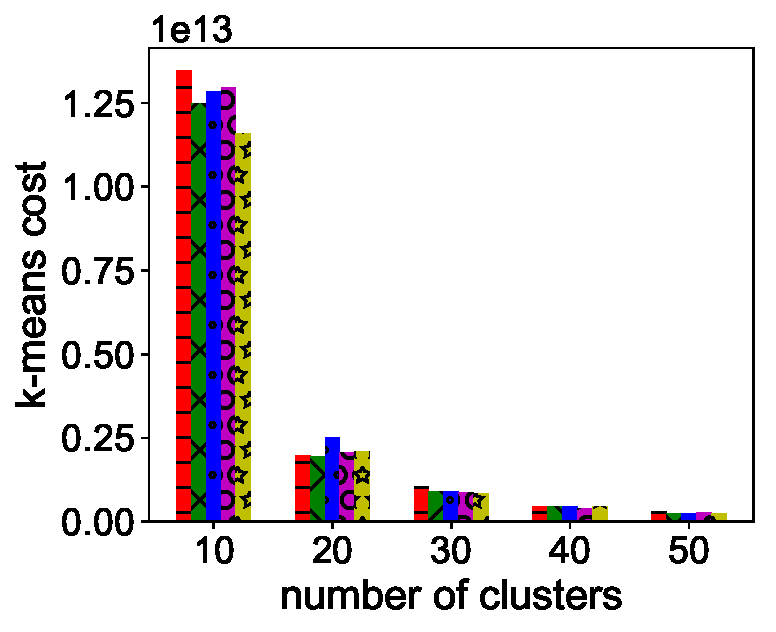
\includegraphics[width=0.24\textwidth]{expfigs/accuracy_k/intrusion_cost_vs_k.pdf}
  }
  \subfloat[\drift]{
  		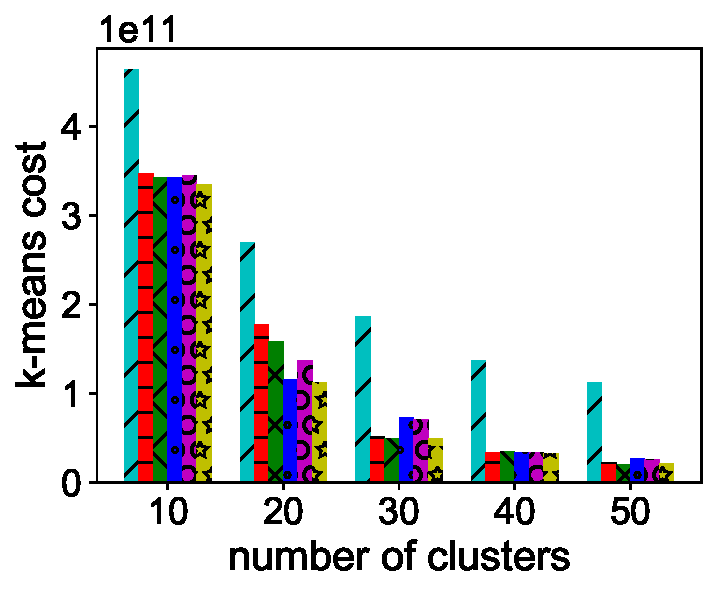
\includegraphics[width=0.24\textwidth]{expfigs/accuracy_k/synthetic_cost_vs_k.pdf}
  }
  \caption{\km cost vs. number of clusters $k$. The cost is computed at the end of observing all the points.  
\km cost of \seqkm on \intrusion dataset is not shown in Figure (c), since it was orders of magnitude larger ($10^4$) than the other algorithms.}
\label{fig:cost-versus-k}
\end{figure*}
%----------------


%----------------
\begin{figure*}
  \centering
  \subfloat[\covtype]{
  \centering 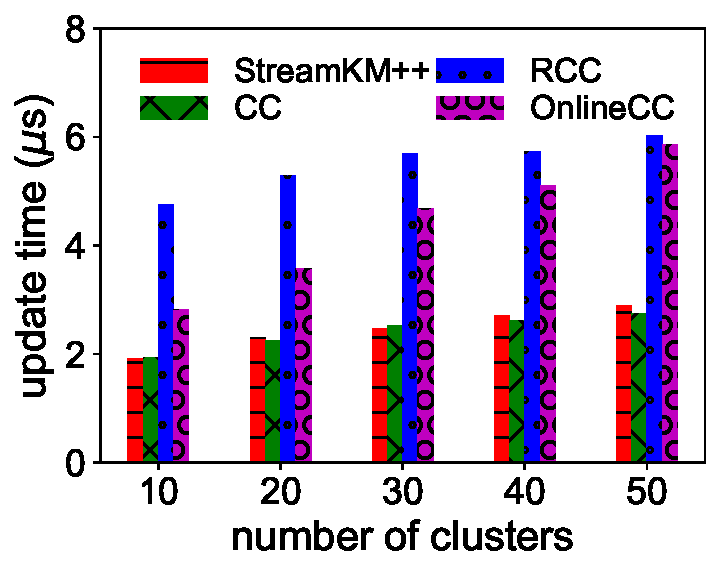
\includegraphics[width=0.23\textwidth]{expfigs/updatetime_k/covtype_update_vs_k.pdf}
  }
  \subfloat[\power]{
  \centering 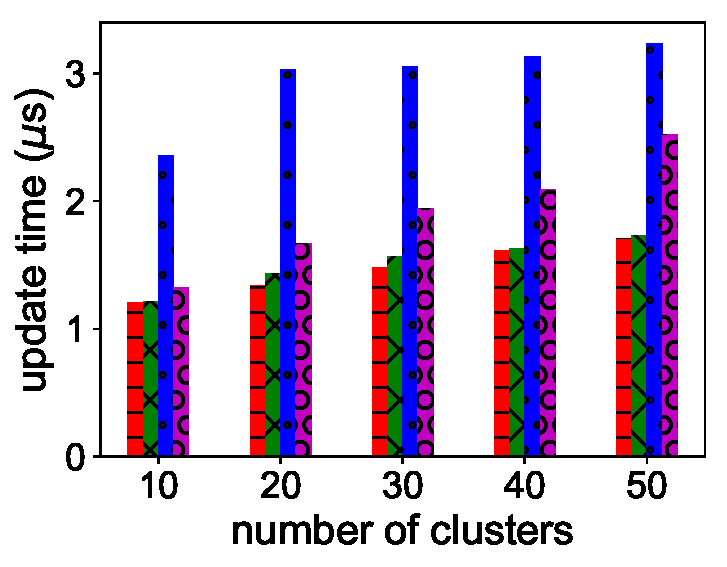
\includegraphics[width=0.23\textwidth]{expfigs/updatetime_k/power_update_vs_k.pdf}
  }
  \subfloat[\intrusion]{
  \centering 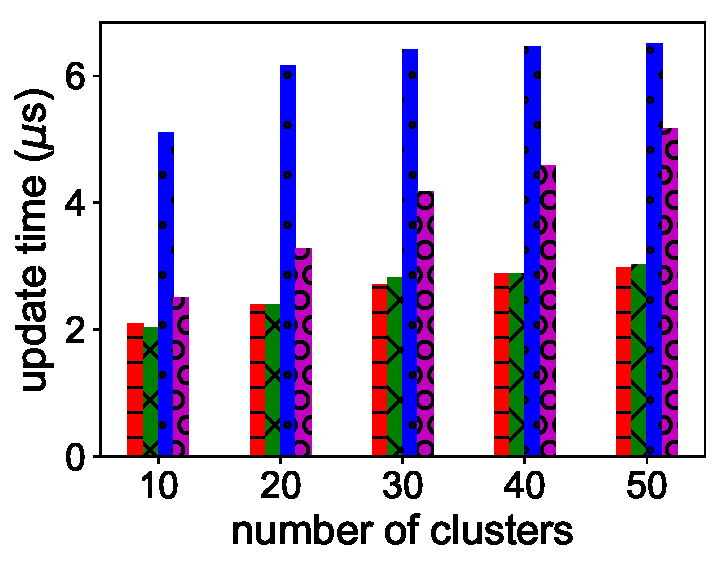
\includegraphics[width=0.23\textwidth]{expfigs/updatetime_k/intrusion_update_vs_k.pdf}
  }
  \subfloat[\drift]{
  \centering 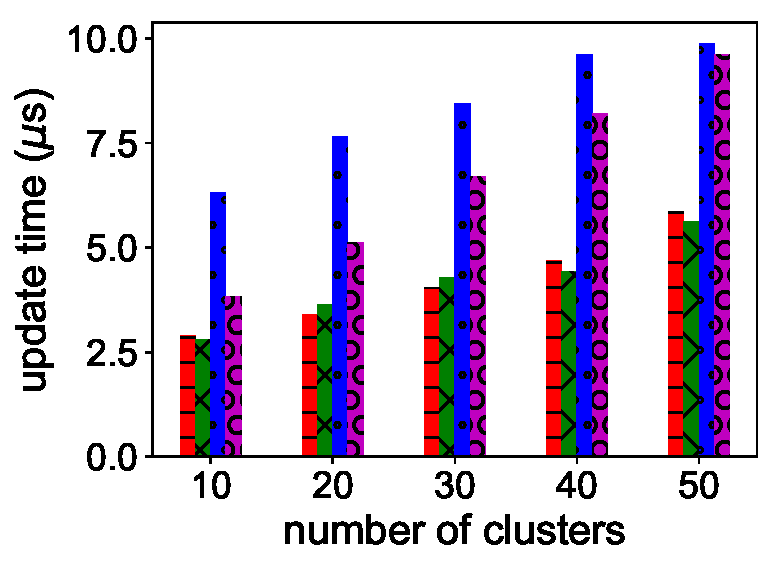
\includegraphics[width=0.23\textwidth]{expfigs/updatetime_k/synthetic_update_vs_k.pdf}
  }
  \caption{Average update time per point (microseconds)  vs. number of clusters $k$. The query interval $q$ is $100$ points.}
  \label{fig:update-versus-k}
\end{figure*}
%----------------


%----------------
\begin{figure*}
  \centering
  \subfloat[\covtype]{
  \centering 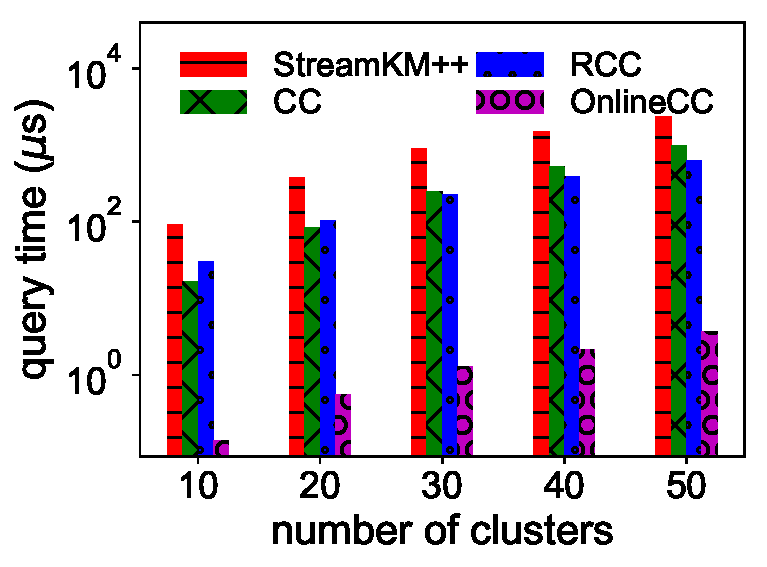
\includegraphics[width=0.23\textwidth]{expfigs/querytime_k/covtype_query_vs_k.pdf}
  }
  \subfloat[\power]{
  \centering 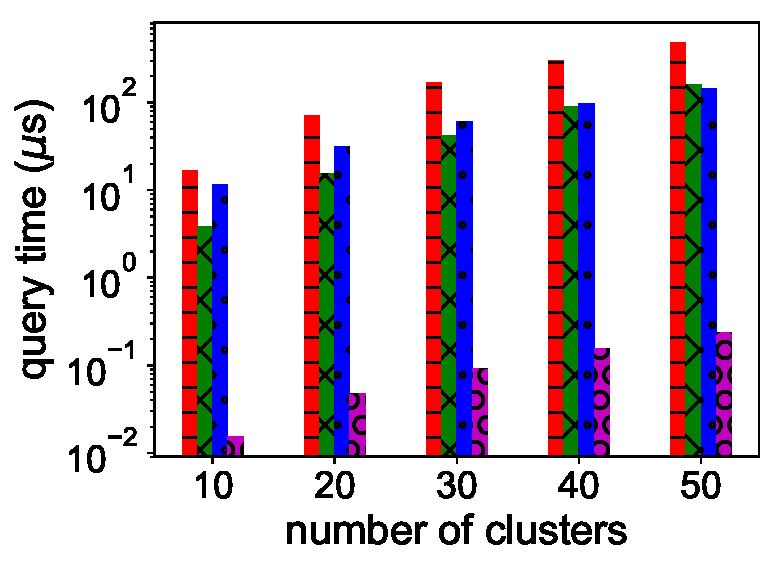
\includegraphics[width=0.23\textwidth]{expfigs/querytime_k/power_query_vs_k.pdf}
  }
  \subfloat[\intrusion]{
  \centering 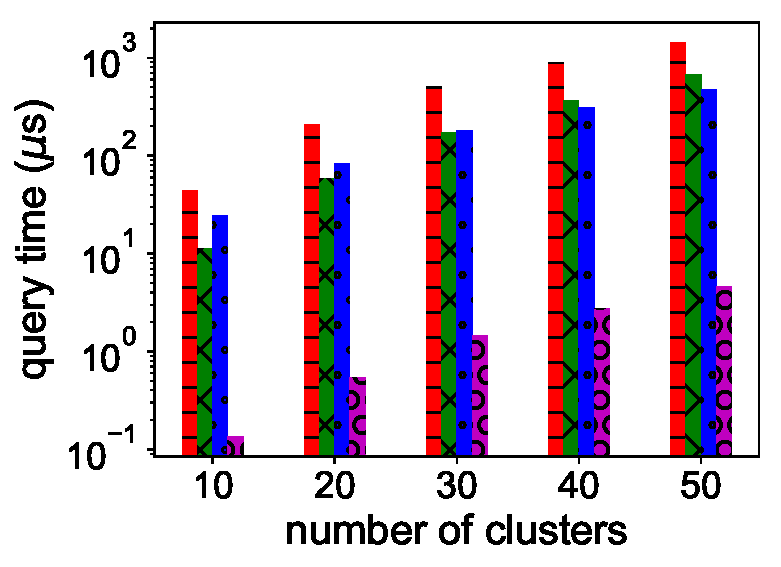
\includegraphics[width=0.23\textwidth]{expfigs/querytime_k/intrusion_query_vs_k.pdf}
  }
  \subfloat[\drift]{
  \centering 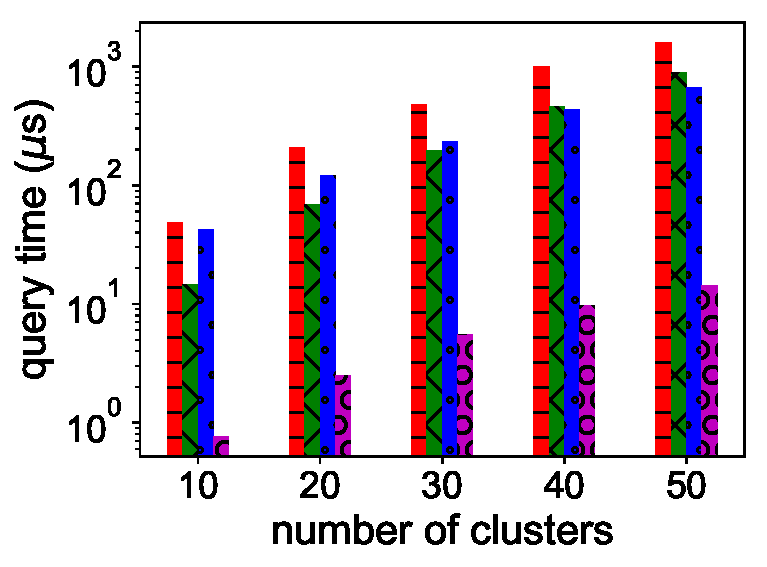
\includegraphics[width=0.23\textwidth]{expfigs/querytime_k/synthetic_query_vs_k.pdf}
  }
  \caption{Average query time per point (microseconds) vs. number of clusters $k$. The query interval $q$ is $100$ points.}
\label{fig:query-versus-k}
\end{figure*}
%----------------


%----------------
\begin{figure*}
  \centering
  \subfloat[\covtype]{
  \centering 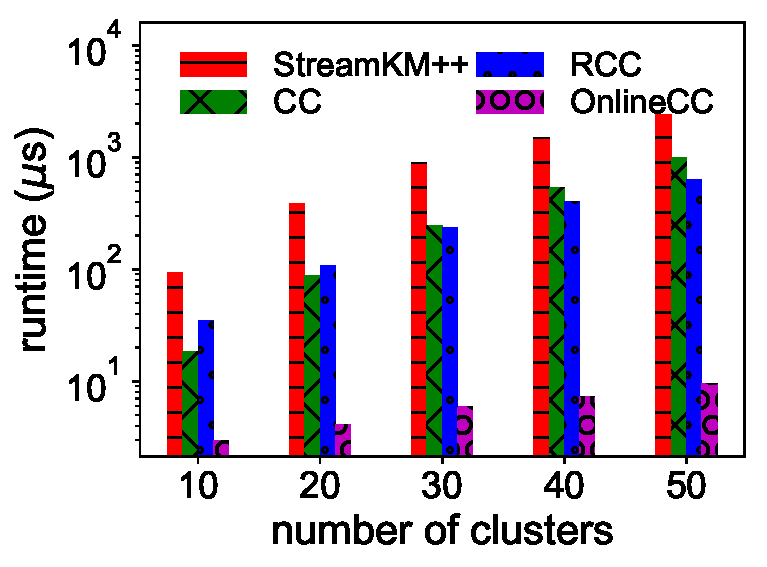
\includegraphics[width=0.23\textwidth]{expfigs/totaltime_k/covtype_total_vs_k.pdf}
  }
  \subfloat[\power]{
  \centering 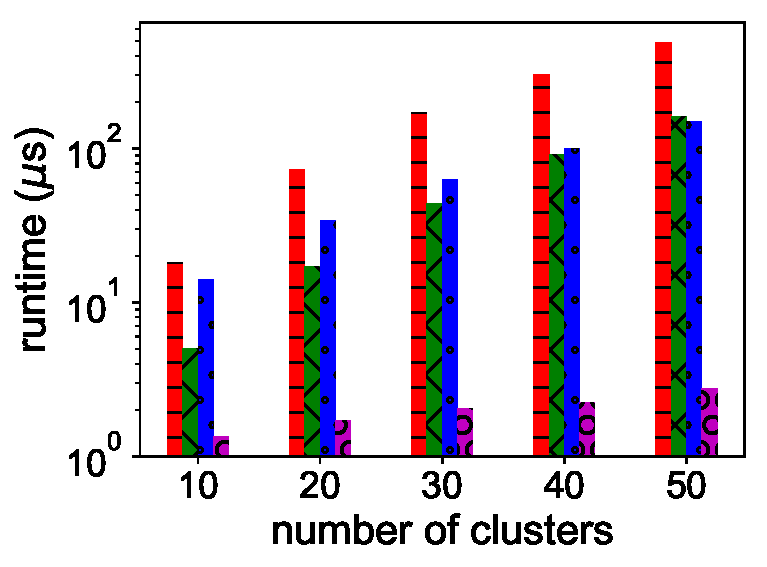
\includegraphics[width=0.23\textwidth]{expfigs/totaltime_k/power_total_vs_k.pdf}
  }
  \subfloat[\intrusion]{
  \centering 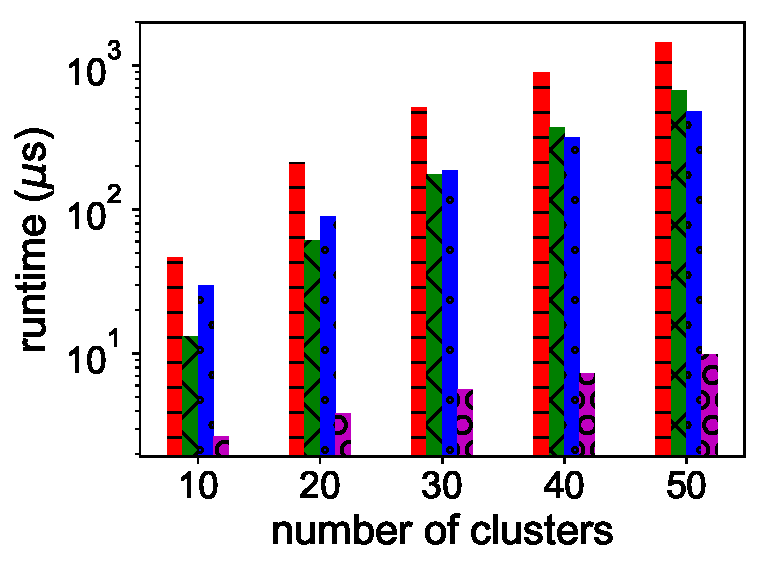
\includegraphics[width=0.23\textwidth]{expfigs/totaltime_k/intrusion_total_vs_k.pdf}
  }
  \subfloat[\drift]{
  \centering 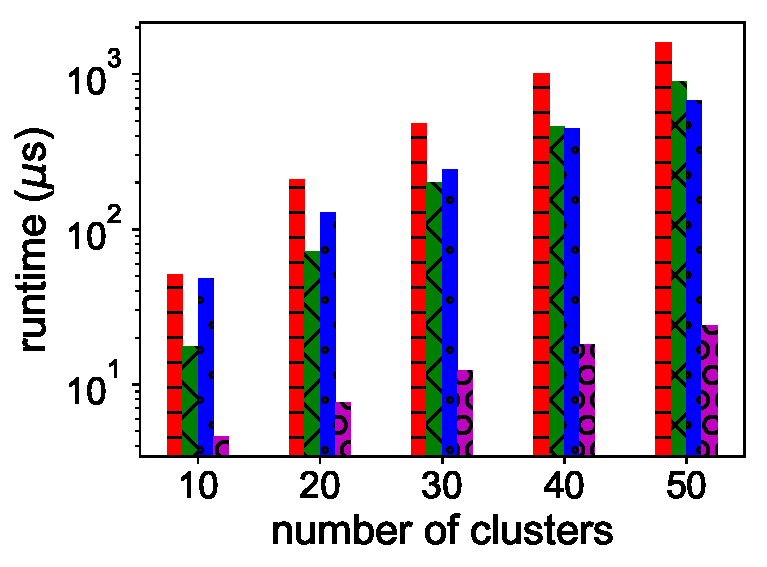
\includegraphics[width=0.23\textwidth]{expfigs/totaltime_k/synthetic_total_vs_k.pdf}
  }
  \caption{Average runtime per point (microseconds) vs. number of clusters $k$. The runtime is sum of average update time (per point) and the average query time (per point). The query interval $q$ is $100$ points.}
  \label{fig:total-versus-k}
\end{figure*}
%----------------